\documentclass{article}
\usepackage[margin=1in]{geometry}
\usepackage[utf8]{inputenc}
\usepackage[english]{babel}
\usepackage{amssymb}
\usepackage{amsmath}
\usepackage{gensymb}
\usepackage{graphicx}
\usepackage{ragged2e}
\usepackage{blindtext}
\usepackage{setspace}
\usepackage{tabularx}
\setlength{\parindent}{4em}
\setlength{\parskip}{1em}
\renewcommand{\baselinestretch}{1.0}

\title{%
   \Large{Úloha 2 - Generalizace budov} \\
  \large{Algoritmy počítačové kartografie}}
\author{Tomáš Hřebec, Kateřina Obrazová}
\date{Praha 2022}

\begin{document}
\doublespacing
\maketitle

\section{\large{Zadání úlohy}}
\subsection{\small{Povinná část}}
\justifying
\textit{Vstup: Množina budov $B = \{B_{i}\}_{i=1}^n$, budova $B_{i} = \{P_{i,j}\}_{j=1}^m$.}
\vspace{0.2cm}\\
\textit{Výstup: G($B_{i}$).}
\vspace{0.2cm}\\
Ze souboru načtěte vstupní data představovaná lomovými body budov. Pro tyto účely použijte vhodnou datovou sadu, např. ZABAGED.
\vspace{0.2cm}\\
Pro každou budovu určete její hlavní směry metodami:
\begin{itemize}
    \item Minimum Area Enclosing Rectangle,
    \item Wall Average.
\end{itemize}
U první metody použijte některý z algoritmů pro konstrukci konvexní obálky. Budovu nahraďte obdélníkem se středem v jejím těžišti orientovaných v obou hlavních směrech, jeho plocha bude stejná jako plocha budovy. Výsledky generalizace vhodně vizualizujte.
\vspace{0.2cm}\\
Odhadněte efektivitu obou metod, vzájemně je porovnejte a zhodnoťte. Pokuste se identifikovat, pro které tvary budov dávají metody nevhodné výsledky, a pro které naopak poskytují vhodnou aproximaci.
\subsection{\small{Volitelná část}}
Generalizace budov metodou Longest Edge.
\vspace{0.2cm}\\
Implementace další metody konstrukce konvexní obálky.
\vspace{0.2cm}\\
Ošetření singulárního případu při generování konvexní obálky.
\clearpage
\newpage
\section{\large{Konvexní obálka}}
Podmnožina \emph{S} roviny se nazývá konvexní jen tehdy, když pro libovolnou dvojici bodů $p,q \in S$ je úsečka $\overline{\emph{pq}}$ zcela obsažena v \emph{S}. (Obr. 1) Konvexní obálka $\mathcal{CH}(S)$ množiny \emph{S} je nejmenší konvexní množina, která obsahuje \emph{S}. Přesněji řečeno, je to průnik všech konvexních množin, které obsahují \emph{S}. (de Berg a kol. 2008)
\vspace{0.2cm}\\
\[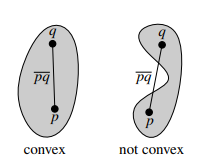
\includegraphics[height=40mm]{images/convex-nonconvex.PNG}\]
\[\textit{\footnotesize{Obr. 1 - Konvexní a nekonvexní podmnožina S}}\\\]
Konvexní obálka \emph{P} je konvexním mnohoúhelníkem. Způsob, jak znázornit mnohoúhelník, je vypsat jeho vrcholy ve směru hodinových ručiček s libovolným počátkem. Chceme tedy vyřešit problém: dáme-li množinu \emph{P} = $\{p_{1}, p_{2} ..., p_{n}\}$ bodů v rovině, vypočtěte seznam, který obsahuje ty body z \emph{P}, které jsou vrcholy $\mathcal{CH}(P)$, uvedené ve směru hodinových ručiček.(de Berg a kol. 2008)
\vspace{0.2cm}\\
\[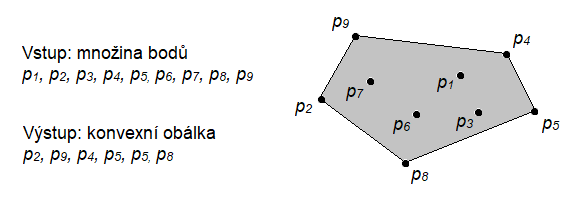
\includegraphics[height=30mm]{images/computing-convex-hull.PNG}\]
\[\textit{\footnotesize{Obr. 2 - Výpočet konvexní obálky}}\]
Při návrhu algoritmu pro výpočet konvexní obálky, se hovoří o průniku všech konvexních množin obsahujících \emph{P}, kterých je nekonečně mnoho. Užitečnější je pozorování, že $\mathcal{CH}(P)$ je konvexní mnohoúhelník. Dále chceme zjistit, jaké jsou okraje $\mathcal{CH}(P)$. Oba koncové body \emph{p} a \emph{q} takové hrany jsou body \emph{P}, a pokud nasměrujeme přímku skrz \emph{p} a \emph{q} tak, že $\mathcal{CH}(P)$ leží vpravo, pak všechny body P musí ležet vpravo od této přímky. (Obr.~3) Platí to i obráceně: pokud všechny body $P \setminus \{p, q\}$ leží napravo od nasměrované přímky skrz \emph{p} a \emph{q}, pak $\overline{\rm\emph{pq}}$ je okraj $\mathcal{CH}(P)$. (de Berg a kol. 2008)\\
\[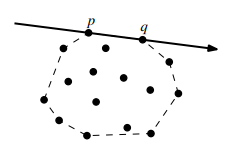
\includegraphics[height=40mm]{images/convex-edges.PNG}\]
\[\textit{\footnotesize{Obr. 3 - Určení hran množiny bodů}}\\\]
\textit{Definice 1: „Konvexní obálka množiny bodů S je množina všech konvexních kombinací bodů bodu S.“}
\vspace{0.2cm}\\
\textit{Definice 2: „Konvexní obálka množiny bodů S je průsečíkem všech konvexních množin, které obsahují S.“}
\vspace{0.2cm}\\
\textit{Definice 3: „Konvexní obálka konečné množiny S v rovině je nejmenším konvexním mnohoúhelníkem $P$,}\\
\indent\indent\indent\textit{~ který obklopuje S. Nejmenší v tom smyslu, že neexistuje žádný další mnohoúhelník $P'$ takový,}\\
\indent\indent\indent\textit{~ že $P \supset P' \supseteq S$.“}
\vspace{0.2cm}\\
\textit{Definice 4:„Konvexní obálka konečné množiny bodů S v rovině je uzavřený konvexní mnohoúhelník $P$}\\
\indent\indent\indent\textit{~ s nejmenší plochou a nejmenším obvodem.“}
\vspace{0.2cm}\\
\textit{Definice 5: „Konvexní obálka množiny bodů S v rovině je sjednocením všech trojúhelníků určených}\\
\indent\indent\indent\textit{~ body v S.“(O'Rourke 1998, str. 65)}
\subsection{\small{Metody konstrukce konvexní obálky}}
Pro konstrukci konvexní obálky se nejčastěji používají:
\begin{itemize}
    \item Inkrementální algoritmy,
    \item Jarvis Scan (Gift Wrapping Algorithm),
    \item Graham Scan,
    \item Quick Hull,
    \item Sweep line (zametací přímka) a plane-sweep,
    \item Divide and Conquer.
\end{itemize}
Některé z těchto algoritmů lze použít pouze pro 2D (Graham Scan), další však i pro více dimenzí (Quick Hull). Algoritmy pro vytvoření 2D konvexní obálky mají vždy jako výstup uspořádaný seznam vrcholů tvořících hranici konvexní obálky seřazený ve stejném pořadí jako dříve. V naší úloze budou použity algoritmy Jarvis Scan a Graham Scan, které budou podrobněji rozebrány v kapitole 2.2 a 2.3.\\
U inkrementálních algoritmů vytvoříme konečný výsledek tak, že postupně vkládáme každý objekt vstupu. Při každém vložení tohoto objektu vypočítáme mezivýsledek. Tyto algoritmy nejsou ve 2D optimální, ovšem v praxi mohou být rychlejší než optimální algoritmy. Ve 3D jsou tyto algoritmy optimální. (Bærentzen a kol. 2012)\\
Základní myšlenkou algoritmu Quick Hull je: \textit{„Pro „většinu“ sad bodů je snadné odhodit mnoho bodů jako definitivně uvnitř obálky, a pak se soustředit na ty, které jsou nejblíže hranici obálky.“~(O'Rourke~1998,~str.~70)} Postup algoritmu Quick Hull je nalézt dva odlišné extrémní body, kdy použijeme nejvíce vpravo nejnižší body a nejvíce vlevo nejvyšší body \emph{x} a \emph{y}, které jsou na první pohled zřetelné. Celá obálka se skládá z horní obálky (upper hull) nad \emph{xy} a z dolní obálky (lower hull) pod \emph{xy}. (Obr. 4)\\
\[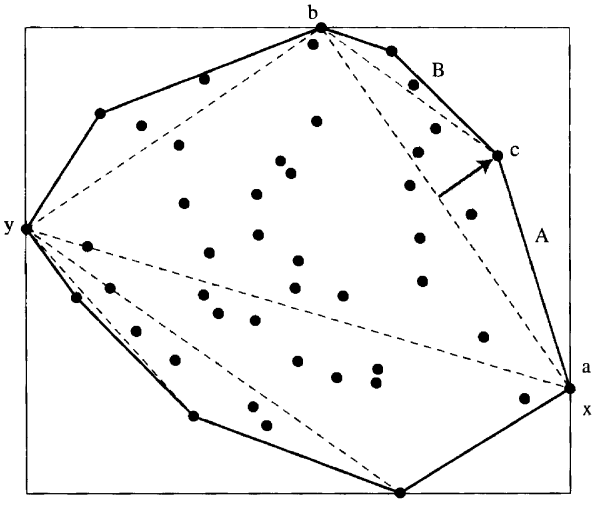
\includegraphics[height=60mm]{images/quickhull.PNG}\]
\[\textit{\footnotesize{Obr. 4 - Quick Hull algoritmus}}\\\]
Obecně funguje Sweep line a plane-sweep tak, že se rozloží vstup na svislé pruhy tak, aby se informace potřebné k vyřešení problému nacházely ve svislých čarách vymezující tyto svislé pruhy. Pro tvorbu konvexní obálky ve 2D existuje algoritmus Sweep line, neboli zametací přímka. (Bærentzen a kol. 2012)\\
Algoritmus Divide and Conquer je optimální v jakékoli dimenzi. \textit{„Při rekurzivním přístupu se rozdělí rekurzivně vstup, dokud nebude možné problém vyřešit triviálně pro danou velikost vstupu. Poté se sloučí řešení dílčích problémů.“ (Bærentzen a kol. 2012, str. 230)}\\
\subsection{\small{Jarvis Scan}}
Dalším algoritmem pro tvorbu konvexní obálky je Jarvis Scan, jenž je nazýván také jako Gift Wrapping algorithm či Jarvis March. Důvodem, proč se tento algoritmus nazývá Gift Wrapping, je následující: \textit{„Lze na to pohlížet jako na omotávání sady bodů provázkem, který ohýbá minimální úhel od předchozí hrany obálky, dokud není sada zasažena.“ (O'Rourke 1998, str. 69)} Algoritmus byl na počátku navržen pro hledání obálek v libovolných rozměrech. Po nějaké době se však přišlo na to, že jej lze implementovat i ve 2D. Předpokladem je, že žádné tři body v \emph{S} nejsou kolineární. Algoritmus je citlivý na velikost vstupních dat, tedy čím menší vstupní data, tím rychleji algoritmus pracuje. Jeho složitost je \emph{O(nh)}, pokud má obálka \emph{h} hran. (O'Rourke 1998)
\vspace{0.2cm}\\
Na Obrázku 5 vidíme průběh tvorby konvexní obálky $P$ pomocí Jarvis Scan algoritmu. Začíná se počátečním bodem (pivotním bodem) $q \in P$, který má minimální souřadnici na ose y. Dále vedeme přímku \emph{p}, která je rovnoběžná s osou x a která prochází bodem \emph{q} ve směru vlevo. Z bodu $q$ hledáme bod svírající maximální úhel $\omega_{max}$ (ve směru hodinových ručiček od \emph{p}). Tomu odpovídá bod $p_{1}$, tudíž $p_{1} \in P$. Z bodu $p_{1}$ hledáme $\omega_{max}$ měřený od $\overline{qp_{1}}$. Tomu odpovídá bod $p_{3}$, tudíž $p_{3} \in P$. Tento postup opakujeme, dokud se konvexní obálka neuzavře v počátečním bodě \emph{q}.\\
\[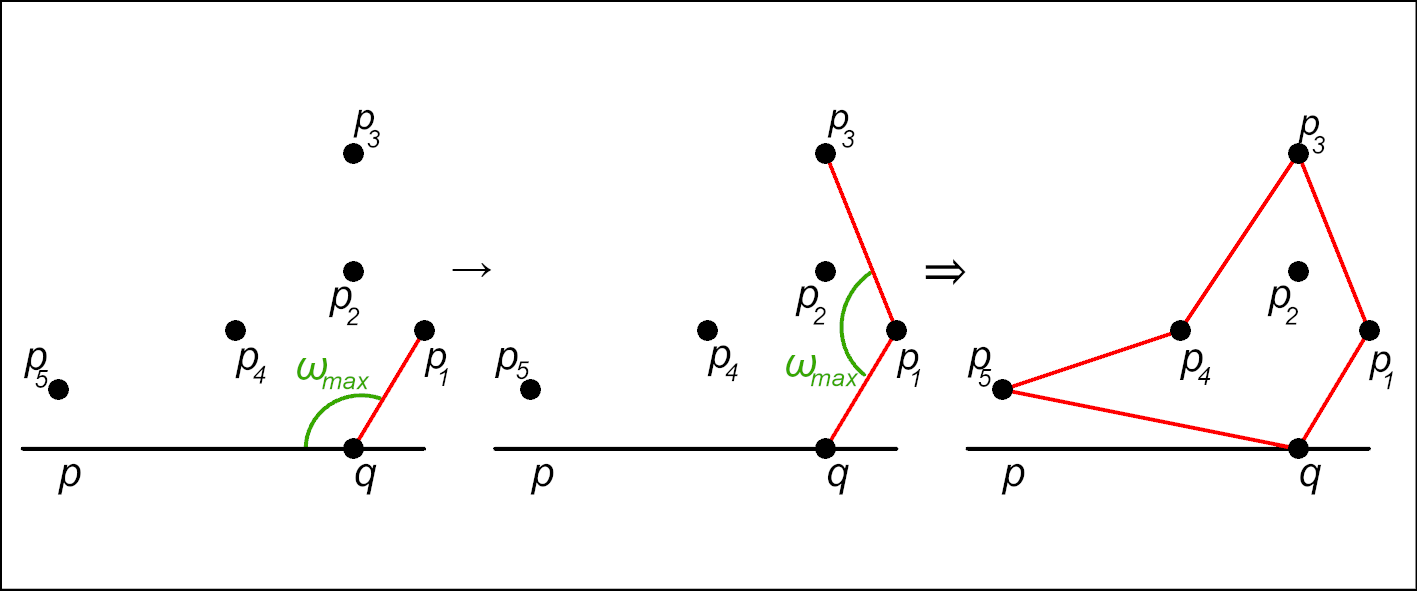
\includegraphics[height=35mm]{images/jarvis-scan.PNG}\]
\[\textit{\footnotesize{Obr. 5 - Jarvis Scan algoritmus}}\\\]
\subsection{\small{Graham Scan}}
Graham Scan je algoritmus sloužící k nalezení obálky bodů ve dvou rozměrech v čase $O(n . log(n))$. Již na počátku algoritmus vyžaduje znát všechny body na vstupu. Začíná se počátečním bodem (pivotním bodem) $q \in P$, který je konstrukcí na hranici konvexní obálky $P$, tedy minimální souřadnicí na ose y. (Obr. 6) Dále se seřadí body podle úhlu vzestupně (při stejném úhlu dvou bodů se bod s menší vzdálenosti od bodu \emph{q} zanedbává). Z bodu \emph{q} vedeme přímku do bodu $p_{1}$, se kterým svírá nejmenší úhel $\omega_{min}$ (proti směru hodinových ručiček). Bod $p_{1} \in P$. Nyní spojíme bod $p_{1}$ s bodem $p_{2}$. Spojení $(q, p_{1}, p_{2})$ je levotočivé, bod $p_{2} \in P$. Bod $p_{2}$ spojíme s bodem $p_{3}$. Spojení $(p_{1}, p_{2}, p_{3})$ je levotočivé, bod $p_{3} \in P$. Dále spojíme bod $p_{3}$ s bodem $p_{4}$. Spojení $(p_{2}, p_{3} ,p_{4})$ je pravotočivé, tudíž bod $p_{3} \notin P$ a z konvexní obálky je vymazán. Vracíme se opět k bodu $p_{2}$, který spojíme s bodem $p_{4}$. Spojení $(p_{1}, p_{2}, p_{4})$ je levotočivé, bod $p_{4} \in P$. Takto se postupuje dokud se konvexní obálka neuzavře. V případě, kdy spojnice mezi body je kolineární, je bod automaticky přidám do konvexní obálky.\\
\[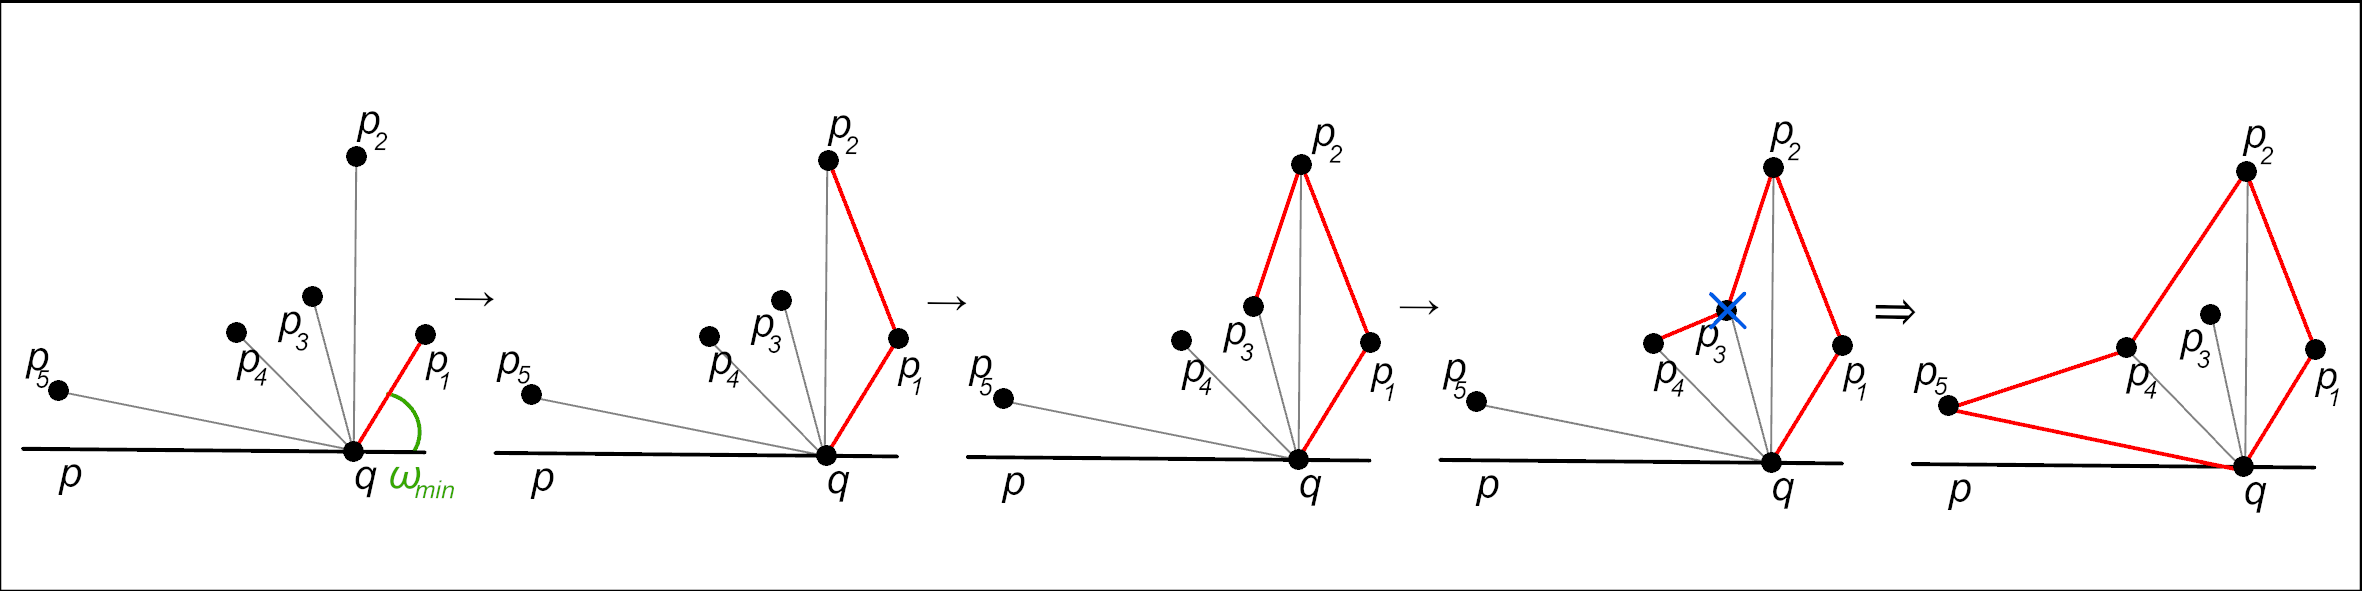
\includegraphics[height=40mm]{images/graham-scan.PNG}\]
\[\textit{\footnotesize{Obr. 6 - Graham Scan algoritmus}}\\\]
\section{\large{Algoritmy pro generalizaci budov}}
V této úloze byly použity pro generalizaci budov algoritmy Minimum Area Enclosing Rectangle, Wall Average a Longest Edge. Všechny tyto algoritmy jsou založeny na hledání hlavního směru budovy (každý jiným způsobem). V momentě, kdy je hlavní směr budovy nalezen, je polygon nahrazen Minimum Bounding boxem (dále jen min-max boxem), který má stejný obsah jako daný polygon a který je natočen do hlavního směru budovy.
\section{\small{Algoritmus Minimum Area Enclosing Rectangle}}
Po vytvoření konvexní obálky $P$ pomocí Jarvis Scan nebo Graham Scan je nutné vytvořit min-max box. Min-max box můžeme popsat jako obdélník $\mathcal{R}$, který obklopuje celou budovu a jehož plocha je minimální. Aby min-max box splňoval tyto podmínky, je potřeba ho opakovaně rotovat okolo množiny bodů $P$ o zápornou směrnici $-\sigma$ určité hrany $P$.\\
Nejprve je třeba vypočítat směrnici hrany konvexní obálky $P$ tvořené body $B = [x_{B}, y_{B}]$ a $C = [x_{C}], y_{C}$:\\
\[tg~\sigma = \frac{x_{C} - x_{B}}{y_{C} - y_{B}}\]
Pomocí matice rotace rotujeme konvexní obálku $P$ o $-\sigma$:\\
\[\begin{bmatrix}
~x~\\~y~\\
\end{bmatrix}
\begin{bmatrix}
~cos(-\sigma) & -sin(-\sigma) \\
~sin(-\sigma) & ~~cos(-\sigma)\\
\end{bmatrix}=
\begin{bmatrix}
~x_{r}~\\~y_{r}~\\
\end{bmatrix}\]
Dále nalezneme extrémní body konvexní obálky $P_{1}, P_{2}, P_{3}, P_{4}$ s extrémními souřadnicemi $\overline{x}, \underline{x}, \overline{y}, \underline{y}$. Tím je možné sestrojit min-max box, jehož strany budou rovnoběžné s osami x a y, a vypočítáme jeho plochu. Tento postup opakujeme pro všechny hrany konvexní obálky. Z tohoto procesu získáme obdélník $\mathcal{R}$ s nejmenší plochou a směrnici hrany konvexní obálky $\sigma_{P}$, z které byl min-max box vytvořen.\\
Dále je třeba detekovat první hlavní směr budovy. Ten představuje u tohoto algoritmu delší ze stran obdélníku~$\mathcal{R}$. Tvar budovy chceme nahradit obdélníkem $\mathcal{R'}$ tak, aby měl stejnou plochu jako generalizovaná budova. Obdélník by měl být úměrně zmenšen a mít společný střed $S$. 
Nyní vypočítáme poměr obdélníků $\mathcal{R}$, $\mathcal{R'}$ (značí se $k$) a plochy obdélníků $A$ (vzniklý min-max box) a $A'$ (zmenšený obdélník):
\[A = ab\]
\[A' = kA = \sqrt{k}a'\sqrt{k}b'\]
Dále vypočítáme uhlopříčky obdélníků $u_{i}$ a $u'_{i}$:
\[\bigg(\frac{\|u_{i}\|}{2}\bigg)^2 = \bigg({\frac{a}{2}}\bigg)^2 + \bigg({\frac{b}{2}}\bigg)^2\]
\[\bigg(\frac{\|u'_{i}\|}{2}\bigg)^2 = k\bigg[\bigg({\frac{a}{2}}\bigg)^2 + \bigg(\frac{b}{2}\bigg)^2\bigg] = k\bigg(\frac{\|u_{i}\|}{2}\bigg)^2\]
Z předchozích vztahů získáme:
\[\|u'_{i}\| = \sqrt{k}\|u_{i}\|\]
Následuje výpočet směrových vektorů pro extrémní body min-max boxu $\Vec{u_{P_{1}}}$, $\Vec{u_{P_{2}}}$, $\Vec{u_{P_{3}}}$, $\Vec{u_{P_{4}}}$:
\[\Vec{u_{P_{1}}} = P_{1} - S\indent\indent\Vec{u_{P_{1}}} = P_{3} - S\]
\[\Vec{u_{P_{1}}} = P_{2} - S\indent\indent\Vec{u_{P_{1}}} = P_{4} - S\]
\vspace{0.3cm}\\
A následně dopočítáme nové vrcholy obdélníku $P'_{1}, P'_{2}, P'_{3}, P'_{4}$:
\[P'_{1} = S + \sqrt{k}\Vec{u_{P_{1}}}\indent\indent P'_{3} = S + \sqrt{k}\Vec{u_{P_{3}}}\]
\[P'_{2} = S + \sqrt{k}\Vec{u_{P_{2}}}\indent\indent P'_{4} = S + \sqrt{k}\Vec{u_{P_{4}}}\]
\section{\small{Algoritmus Wall Average}}
Základním principem algoritmu Longest Edge je uvažovat orientaci každé hrany o zbytek Euklidovského dělení, tedy o $\frac{\pi}{2}$ (vychází výsledek v intervalu $\left[0, \frac{\pi}{2}\right]$)\ a vypočítat průměr těchto směrů, kdy váhou je délka hrany. (Duchéne a kol. 2003)
Na začátku je nutné vypočítat směrnici libovolně zvolené hrany $\sigma'$ a směrnice pro každou hranu budovy $\sigma_{i}$. Následně budou hodnoty $\sigma_{i}$ redukovány o hodnotu $\sigma'$:
\[\Delta\sigma_{i} = \sigma_{i} - \sigma'\]
Z výsledných hodnot $\Delta\sigma_{i}$ vypočítáme zaokrouhlený podíl $k_{i}$:
\[k_{i}~=~\lfloor(\frac{2\Delta\sigma_{i}}{\pi})\rfloor\]
Následuje výpočet zbytku $r_{i}$:
\[r_{i}~=~\Delta\sigma_{i}~–~k_{i}\frac{\pi}{2},\]
kdy \begin{equation}
    r_{i} = \begin{cases}
            < \frac{\pi}{4}; & \text{odchylka od vodorovného směru ($0 \pm \frac{\pi}{2})$}\\
            > \frac{\pi}{4}; & \text{odchylka od svislého směru ($0 \pm \frac{\pi}{2})$}\\
    \end{cases}
\end{equation}
Směr natočení budovy $\sigma$ je dán váženým průměrem $r_{i}$, kde váhou je délka hran $w_{i}$:
\[\sigma = \sigma' + \frac{\sum_{i=1}^{n}r_{i}w_{i}}{\sum_{i=1}^{n}w_{i}}\]
\section{\small{Algoritmus Longest Edge}}
Algoritmus Longest Edge \textit{„měří orientaci nejdelšího okraje budovy po odstranění zarovnaných bodů budovy“. (Duchéne a kol. 2003, str. 2)} Můžeme prohlásit, že první hlavní směr budovy je směrnice nejdelší hrany budovy a druhý hlavní směr je na ni kolmý.
Postup je podobný jako v předchozích algoritmech, kdy je vypočítaná směrnice $\sigma$, konvexní obálka $P$ se otočí o $-\sigma$, avšak v tento moment vytvoříme min-max box a vypočítáme jeho plochu $A$. Dále otočíme konvexní obálku $P$ o úhel $\sigma$, vypočítáme plochu budovy $A'$ a upravíme min.max box tak, aby $A = A'$.
\section{\large{Data}}
Vstupem jsou polygonové vrstvy budov ve formátu \emph{.shp}. Polygonové vrstvy budov byly vybrány z databáze ZABAGED. Výstupem je grafické znázornění polygonů budov a jejich generalizace.
\section{\large{Dokumentace}}
Program je rozdělen do 4 modulů. Modul \emph{Mainform.py} je převážně vygenerován pomocí softwaru QT Creator a slouží k vytvoření uživatelského rozhraní. Modul \emph{algorithm.py} obsahuje algoritmy pro generalizaci budov. Modul \emph{draw.py} slouží především k propojení předešlých dvou modulů a k zajištění vizualizace vstupu a výstupu. Modul \emph{input.py} zajišťuje import vstupních dat v požadovaném formátu.
\subsection{\small{Modul Mainform.py}}
Tento modul obsahuje třídu \texttt{Ui\_Mainform}, která je vytvořena automaticky pomocí QT Creatoru.~(Obr. 7) Tato třída byla posléze doplněna o metody, které se spustí při interakci s uživatelským rozhraním. Jedná se o metody $input$, $simplifyClick$ a $clearClick$. $Input$ vyvolá funkci $loadfile$ z modulu $input.py$ a tím nahraje vstupní polygony ze souboru ve formátu $.shp$ do proměnné $pol\_list$ ve třídě \texttt{Draw}. Metoda \emph{simplifyClick} zajišťuje volání zvoleného algoritmu pro generalizaci budov. Toho je docíleno pomocí odečítání aktuálního itemu v příslušném comboboxu. Tento algoritmus je poté v cyklu spuštěn postupně na všechny vstupní polygony v proměnné $pol\_list$ ze třídy \texttt{Draw}. Jejich generalizace jsou uloženy do proměnné $er\_list$ ve třídě \texttt{Draw}. Poslední metoda \emph{clear} vymaže list, který obsahuje jednotlivé vstupní polygony ($pol\_list$) a list obsahující jejich generalizace ($er\_list$). Tímto odstraní veškeré zobrazované objekty.
\[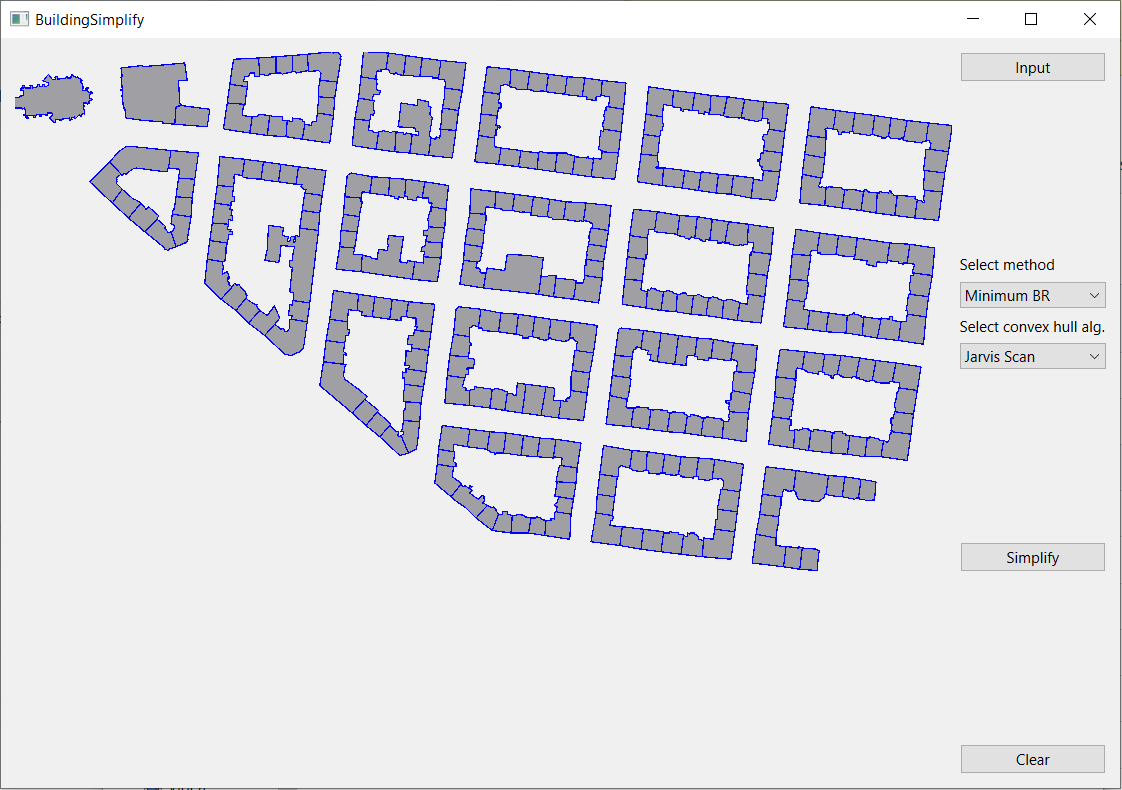
\includegraphics[height=115mm]{images/building-simplify.PNG}\]
\[\textit{\footnotesize{Obr. 7 - Náhled uživatelského rozhraní}}\]
\subsection{\small{Modul input.py}}
Tento modul obsahuje metodu \emph{loadfile}. V této metodě je nejprve načtena cesta ke vstupním datům. Pokud není zvolena žádná cesta, metoda se ukončí. Dále je načten vstupní soubor ve formátu $.shp$. Data z tohoto „shapefilu“ jsou převedeny do formátu \emph{QPolygon}. Následně tato data musí být ještě zobrazena do lokálního souřadnicového systému, který je definován velikostí okna. Takto transformovaná data jsou poté jako jednotlivé polygony vloženy do listu \emph{polygons}, který je posléze touto metodou vracen.
\subsection{\small{Modul draw.py}}
Tento modul obsahuje třídu \texttt{Draw}, kterou dědí od třídy \texttt{QWidget} z knihovny PyQt6. Hlavní funkce tohoto modulu je vykreslovat vstupní a generalizované polygony. Tyto polygony jsou uloženy v listech $pol\_list$ (vstup) a $er\_list$ (generalizace). Toto vykreslení je definováno v metodě \emph{paintEvent}. Poslední dvě metody, \emph{gettery} a \emph{settery}, jsou pro editaci dat z ostatních modulů.
\subsection{\small{Modul algorithm.py}}
Zde se nacházejí jednotlivé algoritmy pro generalizaci budov. Ve třídě \texttt{MinimumAreaEnclosingRectangle} je definován algoritmus Minimum Area Enclosing Rectangle. Tato třída se skládá z devíti metod. První metodou je \emph{get2LinesAngle}, která má na vstupu 4 body ve formátu \emph{QPoint}, které definují dvě úsečky. Metoda vrací velikost úhlu mezi nimi. Metoda \emph{getPointAndLinePosition} má na vstupu 3 body \emph{QPoint}, kde 2 definují přímku a 1 analyzovaný bod. Tato metoda zjistí, ve které polorovině se analyzovaný bod nachází. Výsledek je vracen jako 1 pro bod v levé polorovině, -1 pro bod v pravé polorovině a 0 pro kolineární bod. Další metoda se nazývá \emph{createCHJarvis}, která vytvoří konvexní obálku polygonu pomocí algoritmu Jarvis Scan. Na vstupu je polygon \emph{pol} ve formátu \emph{QPolygon} a výstupem je také konvexní obálka \emph{ch} ve formátu \emph{QPolygon}. Metoda \emph{createCHGraham} je stejná jako předchozí metoda s tím rozdílem, že k tvorbě konvexní obálky využívá algoritmus Graham Scan. Metoda \emph{rotate} má na vstupu \emph{QPolygon} \emph{pol} a úhel \emph{angel} ve formátu \emph{float}. Metoda rotuje vrcholy polygonu o úhel \emph{angel} a vrací jej jako proměnnou $pol\_rot$ ve formátu \emph{QPolygon}. Metoda \emph{minMaxBox} má na vstupu \emph{QPolygon} \emph{pol}, u kterého zjistí jeho min-max box, a následně vypočte obsah tohoto min-max boxu. Tyto hodnoty vrátí jako \emph{S} a $minmax\_box$. Metoda \emph{getArea} vypočte velikost obsahu vstupního QPolygonu. Metoda \emph{resizeRectangle} změní velikost vstupního polygonu \emph{er} tak, aby odpovídala velikosti vstupního polygonu \emph{pol}.\\
Hlavní metoda této třídy se nazývá \emph{minAreaEnclosingRectangle}, která zajišťuje generalizaci vstupního polygonu. Na vstupu je tedy \emph{QPolygon} \emph{pol} a \emph{algorithm}, který představuje zvolený algoritmus pro tvorbu konvexní obálky. Výstupem je generalizovaná budova $er\_new$, ve formátu \emph{QPolygon}. Podrobnější průběh této metody je rozepsán v pseudokódu níže.\\
\vspace{5,5cm}\\
\indent\textit{\textbf{createCHJarvis:}}\\
\indent\textit{Inicializuj prázdnou konvexní obálku ch}\\
\indent\textit{Inicializuj pivota q jako bod s minimální souřadnicí y}\\
\indent\textit{Inicializuj $p_{j}$ jako q a $p_{j-1}$ jako bod, kde $x = q.x~\-~10a,~y = q.y$}\\
\indent\textit{Přidej q do ch}\\
\indent\textit{\textbf{Dokud} $p_{j-1} \ne q$ (ignoruj při prvním průchodu):}\\
\indent\indent\textit{\textbf{Pro} všechny vstupní body p:}\\
\indent\indent\indent\textit{Zjisti úhel mezi přímkou $p_{j}$, $p_{j-1}$ a přímkou $p_{j}$ a p}\\
\indent\indent\indent\textit{Zapamatuj si bod p definující úsečku s největším úhlem}\\
\indent\indent\textit{Přidej zapamatovaný bod od ch}\\
\indent\indent\textit{Aktualizuj $p_{j-1}$ na $p_{j}$}\\
\indent\indent\textit{Aktualizuj $p_{j}$ na zapamatovaný bod}\\
\indent\textit{Vrať ch.}\\
\vspace{0.2cm}\\
\indent\textit{\textbf{createCHGraham:}}\\
\indent\textit{Inicializuj pivota q jako bod s minimální souřadnicí y}\\
\indent\textit{Získej prioritní frontu bodů p seřazených podle velikosti úhlů mezi přímkou, která prochází bodem q}\\
\indent\textit{a je rovnoběžná s osou x, a přímkou definovanou body q a p}\\
\indent\textit{Inicializuj prázdný zásobník S}\\
\indent\textit{Inicializuj index J na 1}\\
\indent\textit{Zjisti délku prioritní fronty n}\\
\indent\textit{Inicializuj pivota q jako bod s minimální souřadnicí y}\\
\indent\textit{Přidej q do zásobníku S, přidej první prvek z prioritní fortny do S}\\
\indent\textit{\textbf{Dokud} index j < n:}\\
\indent\indent\indent\textit{Zjisti pozici bodu $P_{j}$ z prioritní fronty vůči úsečce definovanou posledními 2 body přidanými}\\
\indent\indent\indent\textit{do zásobníku S}\\
\indent\indent\indent\textit{\textbf{Když} bod $P_{j}$ neleží v pravé polorovině:}\\
\indent\indent\indent\indent\textit{Přidej jej do zásobníku S}\\
\indent\indent\indent\indent\textit{Aktualizuj j na $j = j +1$}\\
\indent\indent\indent\textit{\textbf{Jinak} odeber poslední přidaný prvek do zásobníku S}\\
\indent\textit{Výsledný zásobník S představuje konvexní obálku.}\\
\vspace{0.2cm}\\
\indent\textit{\textbf{minAreaEnclosingRectangle:}}\\
\indent\textit{Vytvoř konvexní obálku ch ze vstupního polygonu}\\
\indent\textit{Inicializuj minimální směrnici min-max boxu na 0}\\
\indent\textit{Inicializuj plochu min-max boxu a jeho reprezentaci na min-max box vytvořen z nenatočeného polygonu}\\
\indent\textit{\textbf{Pro} všechny hrany konvexní obálky:}\\
\indent\indent\indent\textit{Vypočítej směrnici hrany $\sigma_{i}$}\\
\indent\indent\indent\textit{Rotuj konvexní obálku o $\sigma_{i}$}\\
\indent\indent\indent\textit{Vytvoř min-max box rotované konvexní obálky}\\
\indent\indent\indent\textit{Vypočti jeho plochu}\\
\indent\indent\indent\textit{\textbf{Když} je plocha minimální:}\\
\indent\indent\indent\indent\textit{Zapamatuj si plochu, minimální směrnici a rotovaný min-max box}\\
\indent\textit{Rotuj min-max box zpět o minimální nalezenou směrnici}\\
\indent\textit{Změň velikost min-max boxu, aby měl stejnou plochu jako původní polygon}\\
\vspace{0.2cm}\\
V druhé třídě \texttt{WallAverage} jsou definované metody pro výpočet generalizace pomocí algoritmu Wall Average. Tato třída obsahuje pět metod. První čtyři – \emph{rotate, minMaxBox, getArea a resizeRectangle} – jsou stejné jako v předchozí třídě. Poslední metoda \emph{computeWallAverage} bere vstupní polygon \emph{pol} \emph{QPolygon} a aplikuje na něj generalizační algoritmus Wall Average. Výstupem je poté \emph{QPolygon}, který aproximuje vstupní polygon. Podrobnější průběh této metody je rozepsán v pseudokódu níže.\\
\vspace{0.2cm}\\
\indent\textit{\textbf{computeWallAverage:}}\\
\indent\textit{Inicializuj směrnici $sigma$ hrany definovanou prvními 2 body vstupního polygonu}\\
\indent\textit{\textbf{Pro} všechny hrany v polygonu:}\\
\indent\indent\textit{Vypočítej jejich směrnici $\sigma_{i}$}\\
\indent\indent\textit{Redukuj $\sigma_{i}$ podle $\sigma'$}\\
\indent\indent\textit{Vypočítej  $k_{i}$}\\
\indent\indent\textit{Vypočítej zbytek po dělení $r_{i}$}\\
\indent\indent\textit{Vypočítej velikost aktuální hrany $w_{i}$}\\
\indent\textit{Získej hlavní směr budovy $\sigma$}\\
\vspace{0.2cm}\\
Poslední je třída \texttt{LongestEdge}, která definuje metody pro generalizaci pomocí algoritmu Longest Edge. Znovu obsahuje metody \emph{minMaxBox, getArea, rotate} a \emph{resizeRectangle}, které jsou opět stejné jako v předchozích třídách. Metoda \emph{getLongestEdgeDirection} vrací směrnici nejdelší hrany ve vstupním polygonu \emph{pol} \emph{QPolygon}. Metoda \emph{computeLongestEdge} aplikuje generalizační metody na vstupní polygon \emph{pol} \emph{QPolygon} a vrací jeho aproximaci $mmb\_new$ \emph{QPolygon}. Podrobnější průběh této metody je rozepsán v pseudokódu níže.\\
\vspace{0.2cm}\\
\indent\textit{\textbf{getLongestEdgeDirection:}}\\
\indent\textit{Inicializuj velikost nejdelší hrany na -1}\\
\indent\textit{\textbf{Pro} všechny hrany ve vstupním polygonu:}\\
\indent\indent\textit{Vypočítej velikost hrany}\\
\indent\indent\textit{\textbf{Když} je velikost hrany větší než nejdelší hrana:}\\
\indent\indent\indent\textit{Aktualizuj velikost nejdelší hrany}\\
\indent\indent\indent\textit{Zapamatuj si startovní a koncový bod aktuální hrany}\\
\indent\textit{Získej hlavní směr budovy jako směrnici nejdelší zapamatované hrany}\\
\vspace{10cm}\\
\section{\large{Porovnání algoritmů}}
Bylo provedeno testování algoritmů na datasetech $Branik.shp, Kamyk.shp$ a $Zbraslav.shp$ o obsahu každého 100 budov. Budovy byly hodnoceny vizuálně, jedná se tedy o subjektivní hodnocení. Výsledný poměr správně vyhodnocených budov ku celkovému počtu budov je uveden v Tabulce 1 v procentech.
\[\begin{tabular}{|p{5.8cm}|{3cm}|{3cm}|{3cm}|}
 \hline
 Algoritmus & oblast Braníku & oblast Kamýku & oblast Modřan \\ 
 \hline
 Minimum Area Enclosing Rectangle & $94\%$ & $96\%$ & $96\%$ \\
 \hline
 Wall Average & $97\%$ & $98\%$ & $98\%$ \\
  \hline
 Longest Edge & $92\%$ & $97\%$ & $92\%$ \\
 \hline
\end{tabular}\]
\[\textit{\footnotesize{Tabulka 1 - Úspěšnost algoritmů pro datasety Branik.shp, Kamyk.shp a Zbraslav.shp}}\\\]
Pro algoritmus Minimum Area Enclosing Rectangle byly problematické budovy, jejichž tvar obsahoval písmeno Z (Obr. 9) a nebo složitější komplex (Obr. 10). Naopak si velmi dobře poradil s budovami ve tvaru U (Obr.~11)
\[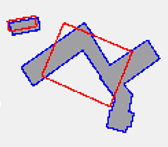
\includegraphics[height=50mm]{images/MAER_9.PNG}\]
\[\textit{\footnotesize{Obr. 9 - Výsledná generalizace algoritmu Minimum Area Enclosing Rectangle}}\\\]
\[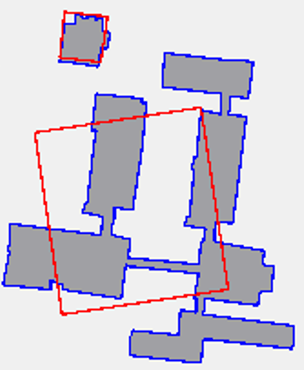
\includegraphics[height=80mm]{images/MAER_10.PNG}\]
\[\textit{\footnotesize{Obr. 10 - Výsledná generalizace algoritmu Minimum Area Enclosing Rectangle}}\\\]
\[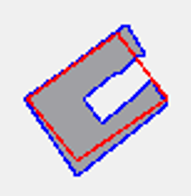
\includegraphics[height=30mm]{images/MAER_11.PNG}\]
\[\textit{\footnotesize{Obr. 11 - Výsledná generalizace algoritmu Minimum Area Enclosing Rectangle}}\\\]
Algoritmus Wall Average měl problém s budovami podobné tvaru L (Obr. 12) nebo E (Obr. 13). 
\[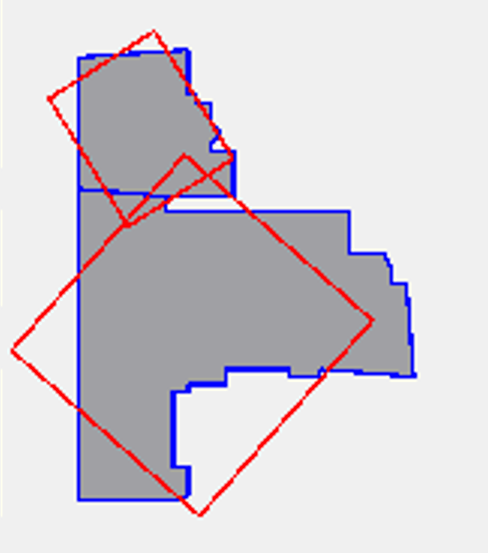
\includegraphics[height=60mm]{images/WA_12.PNG}\]
\[\textit{\footnotesize{Obr. 12 - Výsledná generalizace algoritmu Wall Average}}\\\]
\[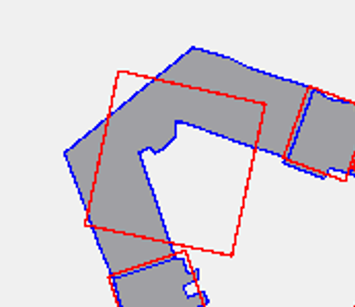
\includegraphics[height=60mm]{images/WA_13.PNG}\]
\[\textit{\footnotesize{Obr. 13 - Výsledná generalizace algoritmu Wall Average}}\\\]
Algoritmus Longest Edge měl problémy například u budovy ve tvaru více rozevřeného U (Obr. 14). 
\[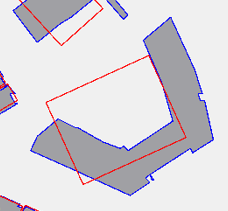
\includegraphics[height=70mm]{images/LE_14.PNG}\]
\[\textit{\footnotesize{Obr. 14 - Výsledná generalizace algoritmu Longest Edge}}\\\]
Na závěr je nutné dodat, že pro jiné datasety se výsledky budou lišit a nelze říci objektivně, který je ten nejlepší. Vždy to bude záviset na orientaci vzhledem k ostatním prvkům mapy. Na závěr v Přílohách naleznete výstupy všech algoritmů pro všechny uvedené datasety.
\clearpage
\newpage
\section{\large{Zdroje}}
BÆRENTZEN, J. A., GRAVESEN, J., ANTON, F., AENÆS, H. (2012): Convex Hulls. In: J. A. Bærentzen, J. Gravesen, F. Anton, H. Aenæs (ed.): Guide to Computational Geometry Processing - Foundations, Algorithms, and Methods. Springer, Londýn, 330 s.\\
DE BERG, M., CHEONG, O., VAN KREVELD, M., OVERMARS, M. (2008): Computational Geometry: Algorithms and Applications. Third Edition. Springer, Berlín, Heidelberg, 388 s.\\
DUCHÉNE, C., BARD, S., BARILLOT, X., RUAS, A., TRÉVISAN, J., HOLZAPFEL, F. (2003): Quantitative and qualitative description of building orientation. Institut Géographique National, Paříž, 11 s.
O'ROURKE, J. (1998): Computational Geometry in C. Second Edition. Cambridge University Press, 392 s.\\
\section{\large{Přílohy}}
Příloha 1 - Výstup algoritmu Minimum Area Enclosing Rectangle pro dataset $Branik.shp$
\[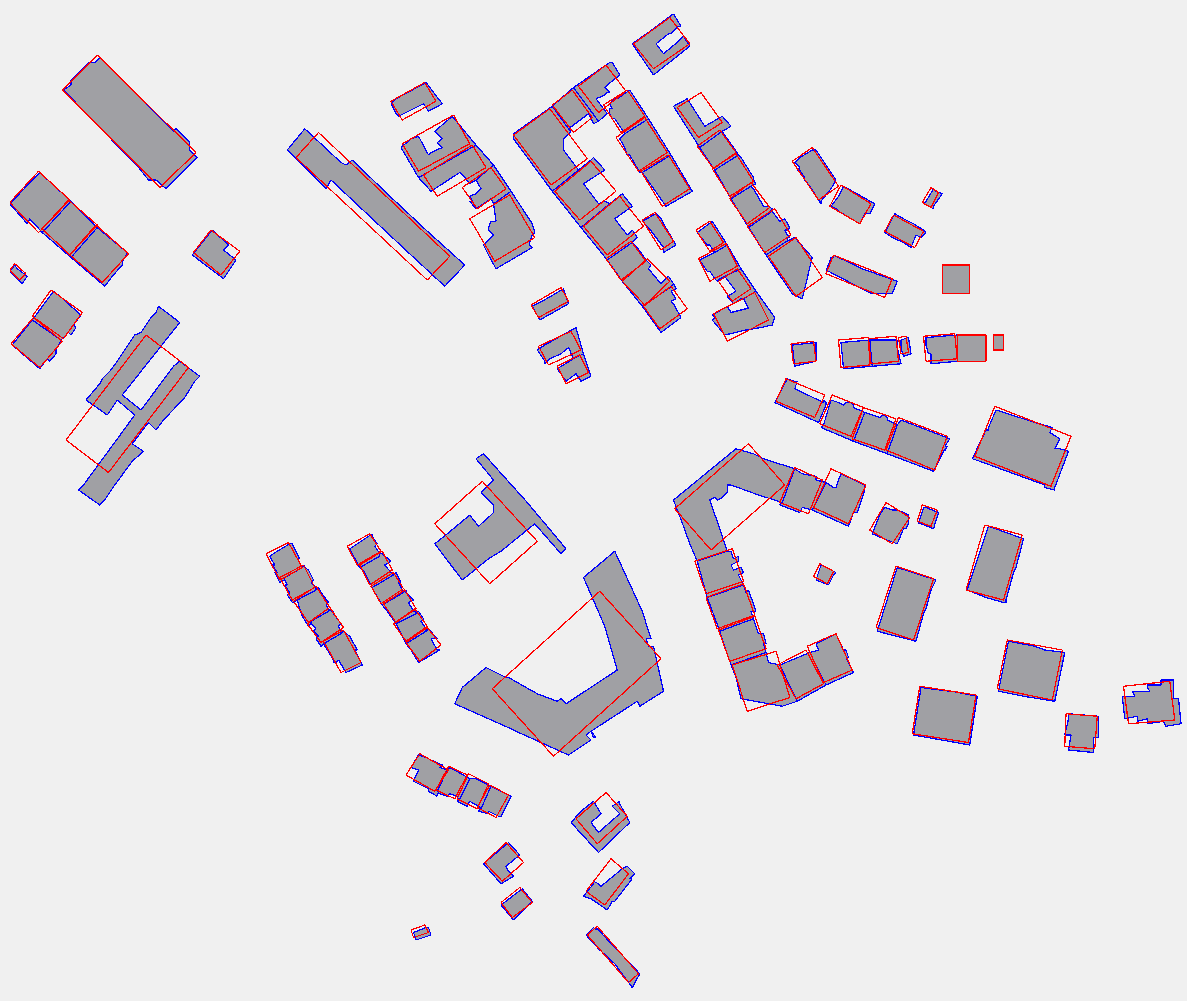
\includegraphics[height=140mm]{images/Branik_MAER.PNG}\]
\clearpage
\newpage
Příloha 2 - Výstup algoritmu Minimum Area Enclosing Rectangle pro dataset $Kamyk.shp$
\[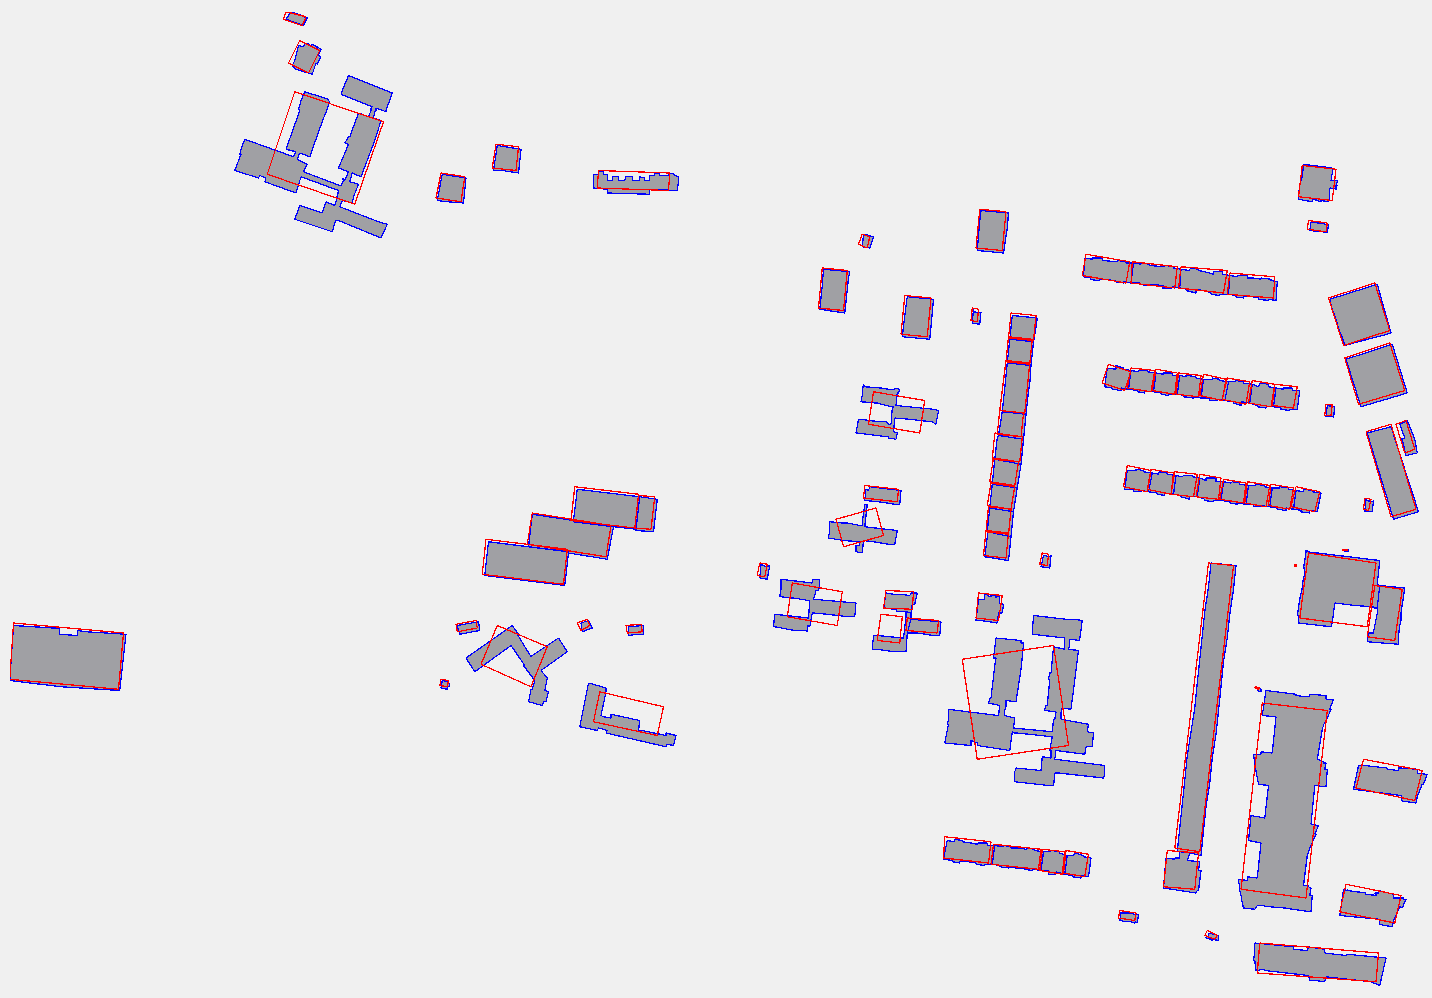
\includegraphics[height=115mm]{images/Kamyk_MAER.PNG}\]
\clearpage
\newpage
Příloha 3 - Výstup algoritmu Minimum Area Enclosing Rectangle pro dataset $Zbraslav.shp$
\[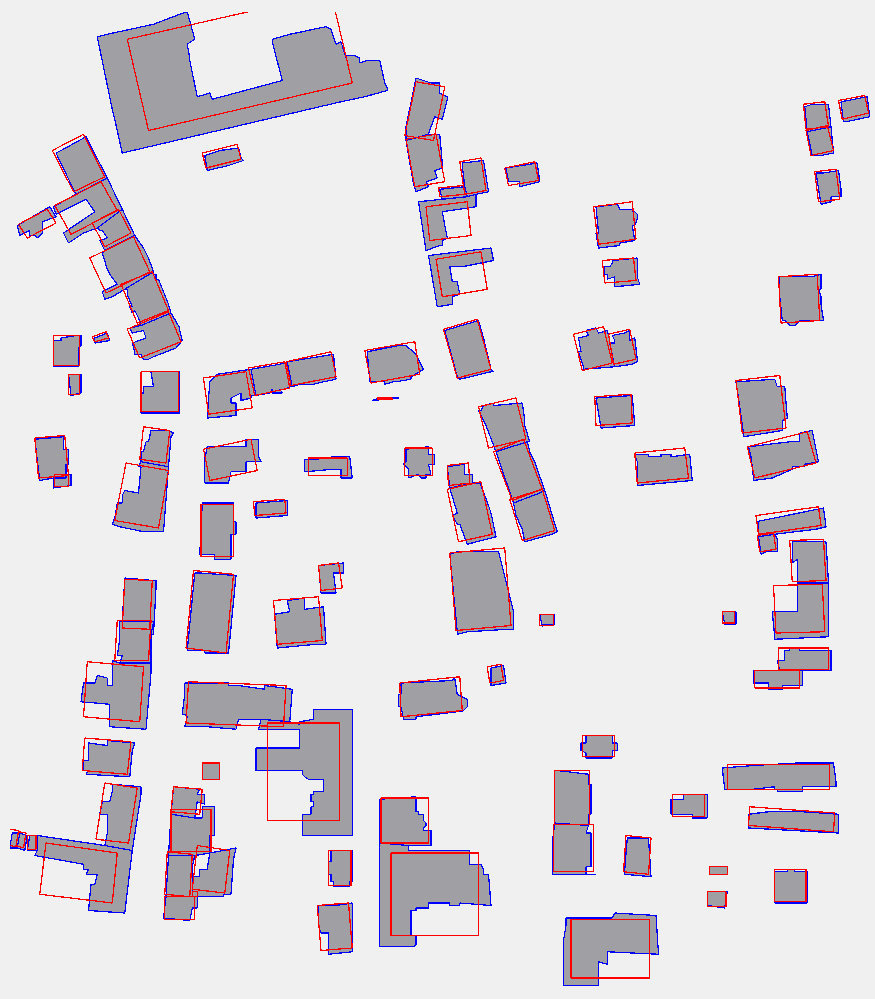
\includegraphics[height=180mm]{images/Zbraslav_MAER.PNG}\]
\clearpage
\newpage
Příloha 4 - Výstup algoritmu Wall Average pro dataset $Branik.shp$
\[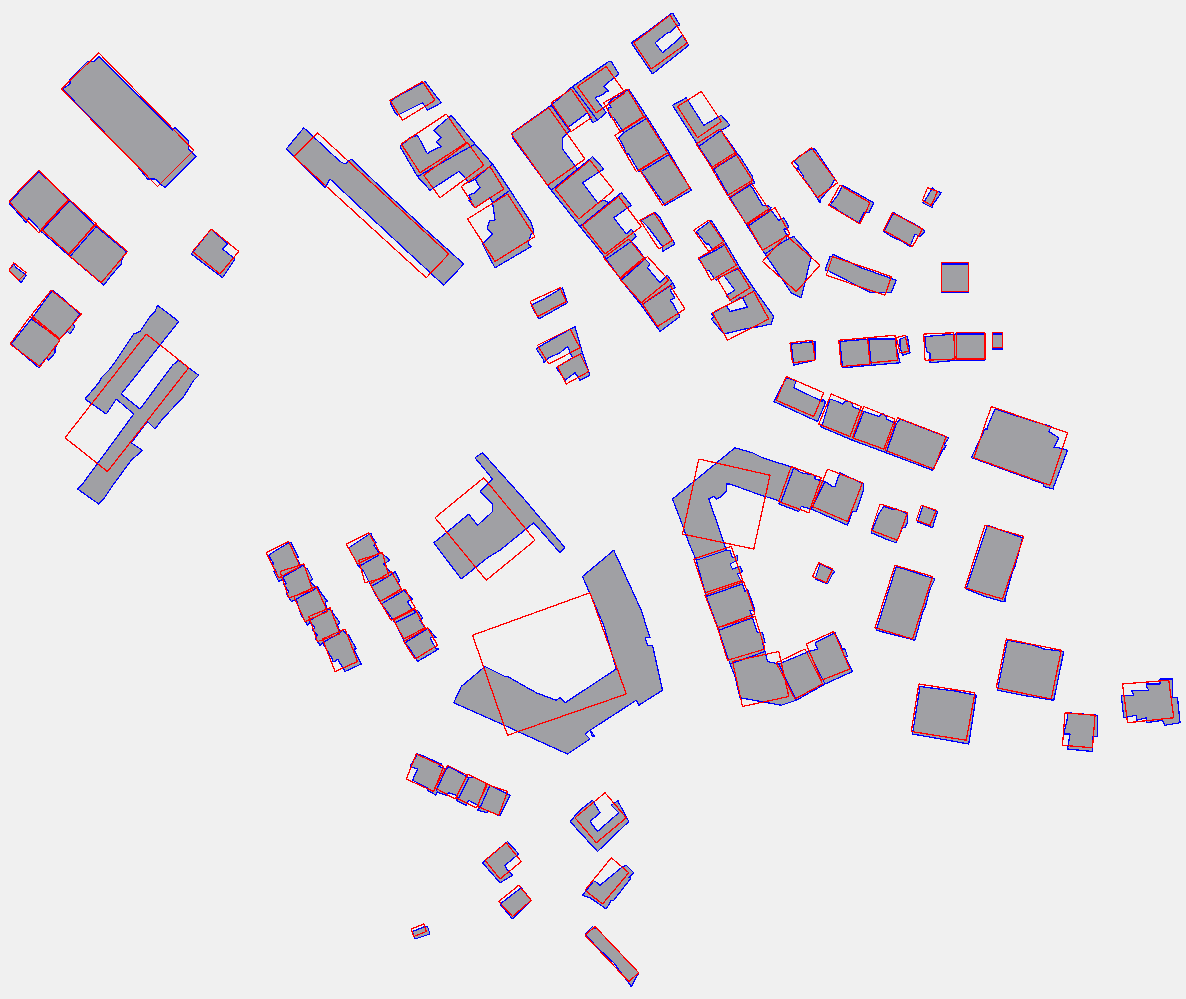
\includegraphics[height=140mm]{images/Branik_WA.PNG}\]
\clearpage
\newpage
Příloha 5 - Výstup algoritmu Wall Average pro dataset $Kamyk.shp$
\[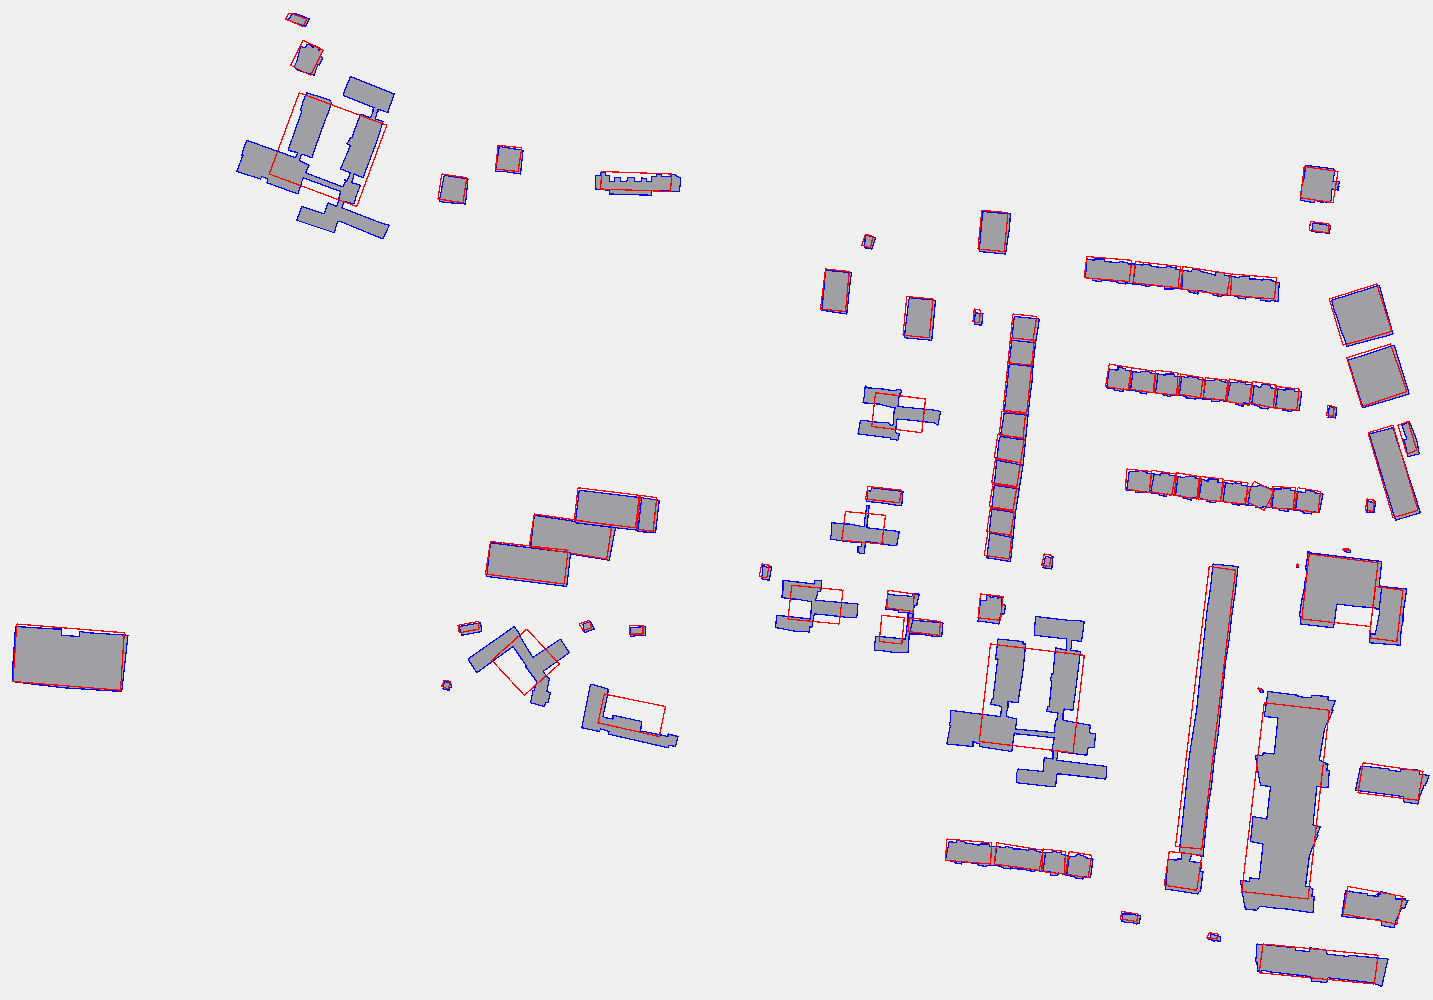
\includegraphics[height=115mm]{images/Kamyk_WA.PNG}\]
\clearpage
\newpage
Příloha 6 - Výstup algoritmu Wall Average pro dataset $Zbraslav.shp$
\[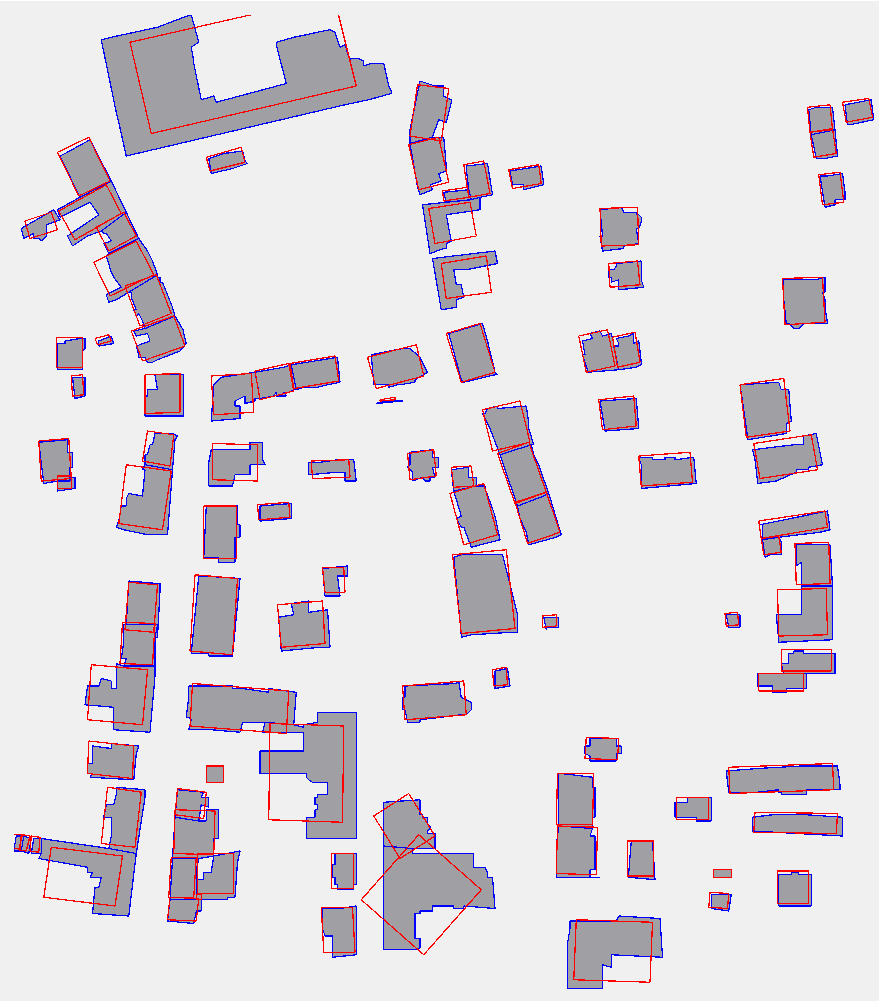
\includegraphics[height=180mm]{images/Zbraslav_WE.PNG}\]
\clearpage
\newpage
Příloha 7 - Výstup algoritmu Longest Edge pro dataset $Branik.shp$
\[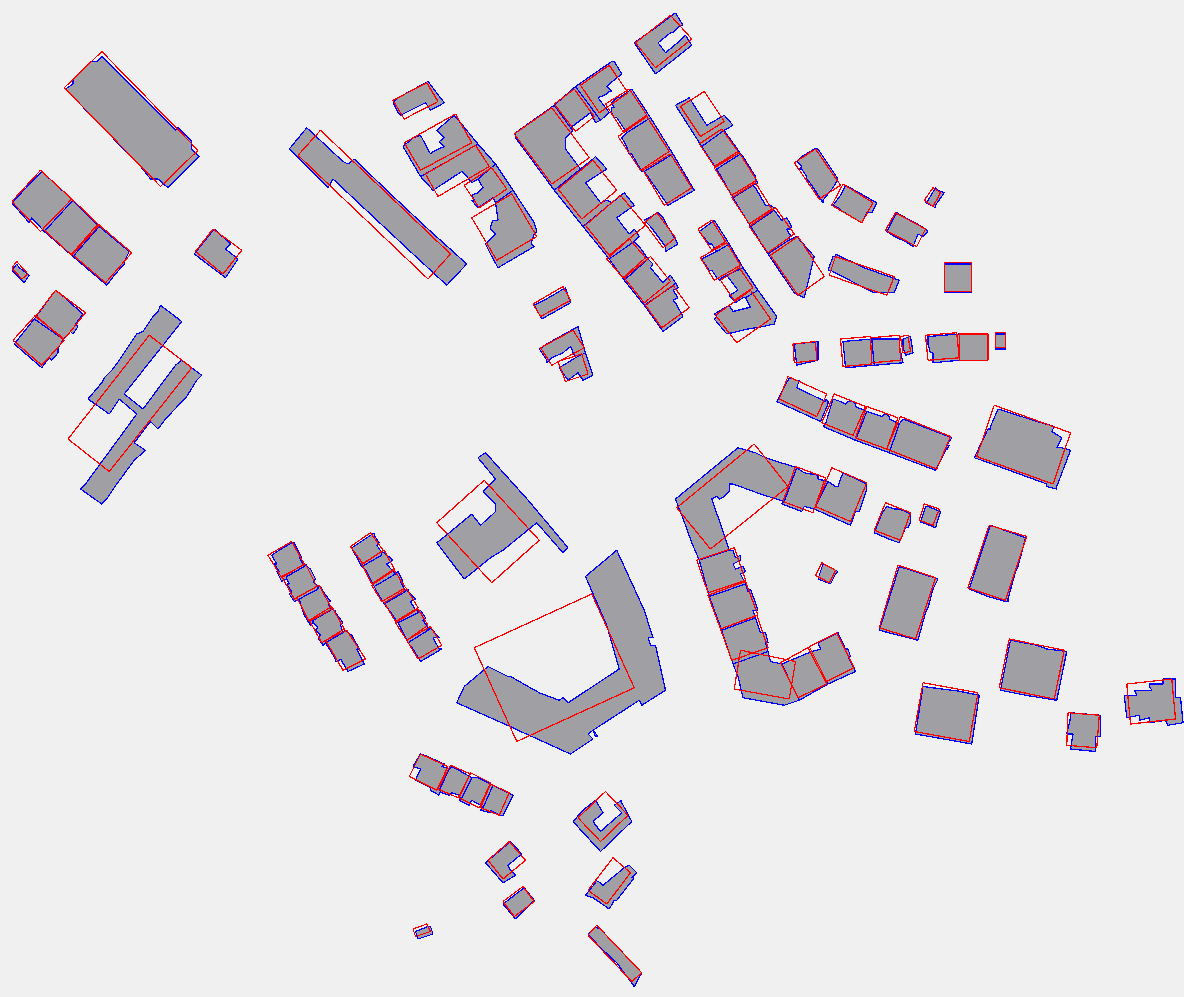
\includegraphics[height=140mm]{images/Branik_LE.PNG}\]
\clearpage
\newpage
Příloha 8 - Výstup algoritmu Longest Edge pro dataset $Kamyk.shp$
\[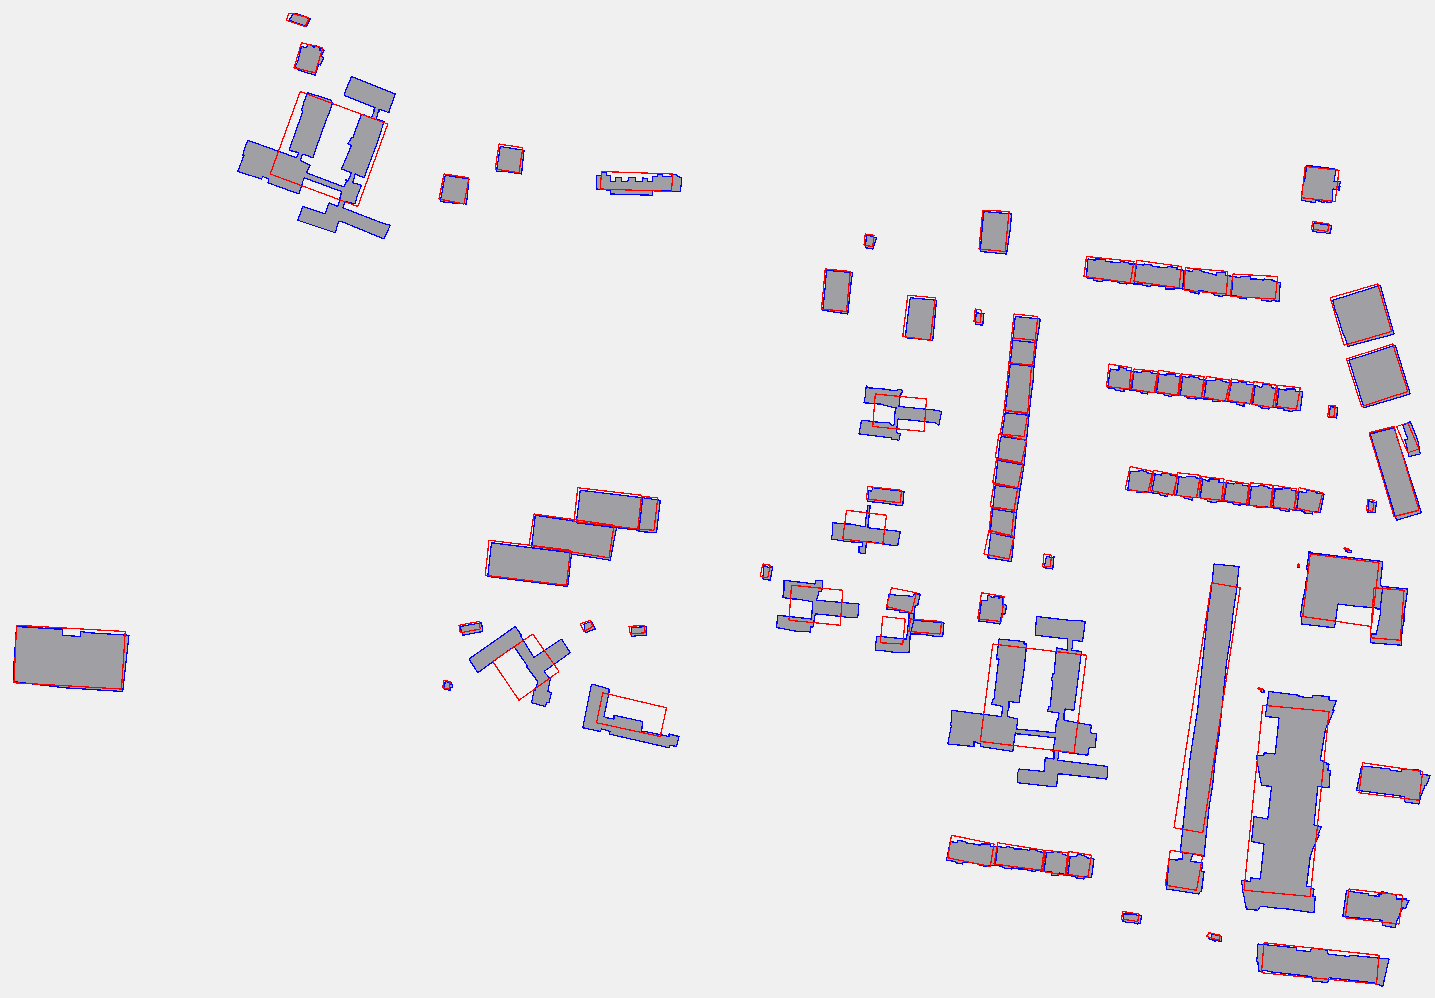
\includegraphics[height=115mm]{images/Kamyk_LE.PNG}\]
\clearpage
\newpage
Příloha 9 - Výstup algoritmu Longest Edge pro dataset $Zbraslav.shp$
\[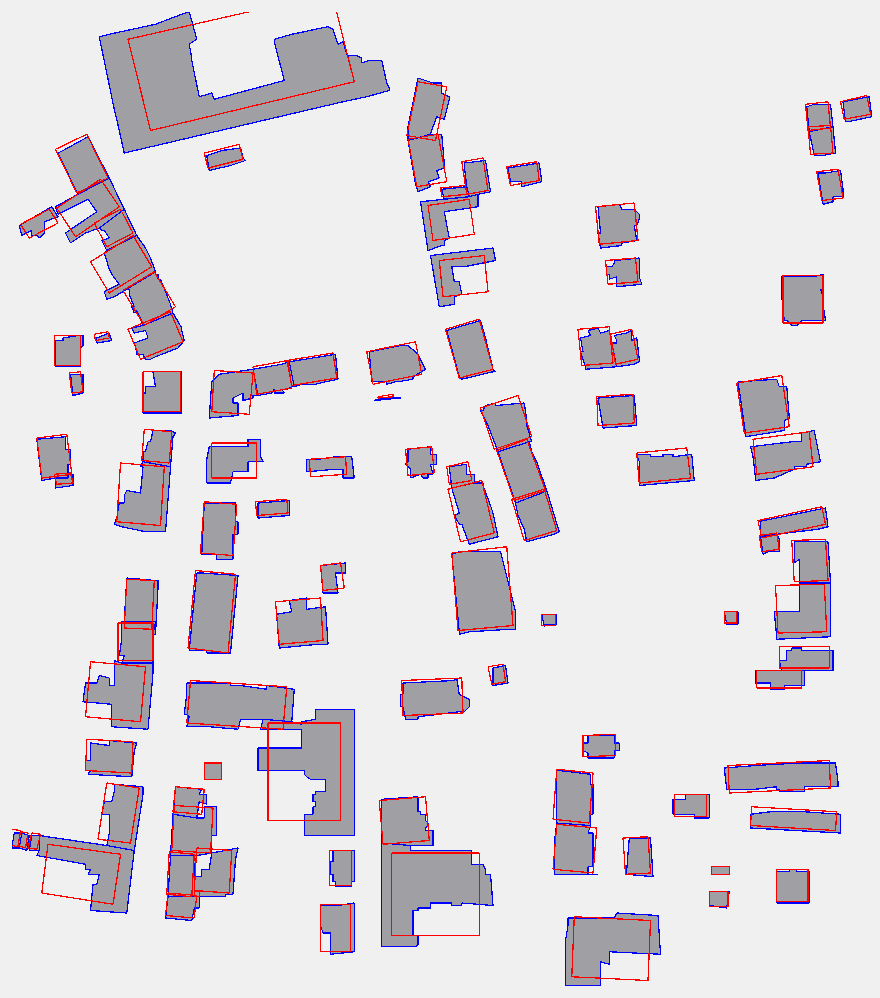
\includegraphics[height=180mm]{images/Zbraslav_LE.PNG}\]
\clearpage
\newpage
\end{document}
